\documentclass{report}

\usepackage[latin1]{inputenc} 
\usepackage[T1]{fontenc}      
\usepackage[english]{babel}  
\usepackage{hyperref}
\usepackage{algorithm}
\usepackage{algorithmic}
\usepackage[top=2cm, bottom=2cm, left=2cm, right=2cm]{geometry}
\usepackage{wrapfig}
\usepackage{graphicx}
\usepackage{caption}
\usepackage{subcaption}

\title{Localization and extraction of centroids from composite materials X-ray tomographies BROUILON}
\author{Mohamed Aymane Benayada \and Thibault Leblanc \and Kai-Wei Tsou \and Julien Zhou}
\date{March 2019}

\begin{document}
 
\maketitle

\tableofcontents


\chapter{Introduction}
 
Increasingly more composite materials are used in aeronautics, especially in engines. These materials are made of 	carbon fibers bundles which are weaved together within a resin matrix. It is essential, especially in ordre to reduce the cost of experimental studies, to determine or even predict the mechanical properties of these new materials thanks to numerical methods. Checking the weaving is necessary in order to discard parts with a defective weaving. Non destructive testing of aeronautic materials uses X-ray tomography to scan the structure of the material.


Currently, those volumes are analyzed manually and the centers of the bundles are annotated manually on a few slices. The remaining annotations are obtained through interpolations.This structure extraction step is currently essential for it allows to define the number of bundles to represent and to identify them to obtain their trajectory.


Manual annotations and interpolation corrections are time consuming and hard to get. To this day, the automation of centroid detection remains an open subject because of the complexity of image interpretation, especially when the bundles are weaved in a very compact way and that is impossible to distinguish them, without taking into consideration their configuration on neighboring slices.\newline

In this project, our objective has been to try an approach to automatize the detection of bundle of fibers in X-ray tomographies. As getting annotated data is want to avoid, we based our approach on mainly unsupervised methods or methods with the least inputs from an external user possible.

In the following, present the database and the way we preprocessed our images before introducing the methods that we implemented and discussing our results.

\chapter{Context}

In this chapter, we introduce a formalization of the problem, the database that will be used in the following to test the approaches and a scoring methodology.

\section{Problem}

The overall objective of the project is to study approaches to automatize the detection and segmentation of different bundles of fibers from X-ray tomographies to retrieve their centroids, the far end objective being to implement a non destructive control procedure.  

In fact, if we manage to get the centroids on each slice of the volume, and to link them between the slices, a 3D model of the material could be derived, which would enables to test the mechanical properties on numerical simulations.

Several classic image processing method enables image segmentation, but they usually work with images with good contrasts and clearly defined edges, which is not really the case here as we will see. To account for that, we tried machine learning and deep learning methods.

\section{Database}

Safran provided us a volume of 1018 slices of 1024x1004 pixels images. \newline

Visualisation of a few images....

In the few firsts and last images, we observed distorsions in the images, so we decided to discard them (at least in the beginning). We kept the images from 150 to 850 (included), totalling 650 images.  

At first view, it seems that the bundles of fibres often not clearly separated of clumped together in the images, we can assume that the main hindrance would be to find a way to separate those clumps.

\section{Scoring: Aggregated Jaccard Index}

We define here a scoring methodology that we will use in the following to evaluate the methods: the Aggregated Jaccard Index. \newline


\href{https://www.researchgate.net/publication/314271512_A_Dataset_and_a_Technique_for_Generalized_Nuclear_Segmentation_for_Computational_Pathology}{source}

The Jaccard index, or Jaccard similarity coefficient, or Intersection over union is a metric used in statistics to compare the similarity between sets.  
For two sets of elements (in our case, it would be pixels), $A$ and $B$, the Jaccard index $J(A,B)$ is defined as:
\[J(A,B)=\frac{|A\bigcap B|}{|A\bigcup B|}\]
This function returns 0 if the two sets have no element in common and 1 if they are identical. \newline

We use a metric inspired from this index, an Aggregated Jaccard Index (AJI), enabling the comparison of different segmentations for unlabeled elements.  
Let's call $G_i$ the ground truth sets and $D_j$ the detected ones. The metric is computed as follows:
\begin{algorithm}
\caption{Computing the Aggregatd Jaccard Index}
\begin{algorithmic} 
\STATE Numerator $N \leftarrow 0$
\STATE Denominator $D \leftarrow 0$
\FOR{Each ground truth bundle $G_i$}
\STATE $j \leftarrow argmax_k J(G_i, S_k)$
\STATE $N \leftarrow N+|G_i\bigcap S_j|$
\STATE $D \leftarrow D+|G_i\bigcup S_j|$
\STATE Mark $S_j$ as used
\ENDFOR
\FOR{Each segmented bundle $S_k$}
\IF{$S_k$ has not been used}
\STATE $D \leftarrow D + |S_k|$
\ENDIF
\ENDFOR
\STATE $AJI \leftarrow N/D$
\end{algorithmic}
\end{algorithm}

For each ground truth object $G_i$, we associate the segmented object $S_j$ and add the pixel count $|G_i\bigcap S_j|$ to AJI numerator and $|G_i\bigcup S_j|$ to the denominator.    
Therefore, for ground truth fibers not detected, it only adds its pixel count to the denominator.   
And besides, the pixel count of all the unused detected element is added to the denominator count. \newline

This index tackle the following errors:
- Missed detection of ground truth annotated objects (pixel count in denominator increased)
- False detection (unused $S_k$, pixel count in denominator)
- Under-segmentation (the pixels are added several times in the denominator)
- Over segmentation (several unused detections and small numerator VS big denominator)

Like before, the score is 1 if the segmentations are identical, and decreases if we are "`far"' from it.

\chapter{Image preprocessing}

In this chapter, we present the methodology used to preprocess the images before the segmentation step.
As written before, the firsts and last images of the volume show some distorsions, therefore, we only took the images from 150 to 850 from the 1018 images provided. \newline

We used the following process:  
- Trimming: in order to only keep the relevant part,  
- Denoising: we applied a first median filter to attenuate the noise,  
- Histogram Manipulation: to enhance the contrast of the image,  
- Denoising: to attenuate the potential noise from the last step.

\section{Trimming}

 The part that interest us in the images is the center.   
Visu

The first step is therefore to separate it from the rest. We roughly extracted a rectangle in the middle of the image, containing the interesting part.
Visu

\section{Denoising}
Blablabla

\section{Histogram Manipulation}

It is possible to increase the contrast of an image by adjusting its histogram.   
We explored 3 histogram manipulation methods:  
- histogram stretching  
- histogram equalization  
- adaptative equalization.  \newline

At the end, the method that we kept is the adaptative equalization.

\subsection{Histogram Stretching}

This technique improves the constrast by stretching the range of intensity to span the whole range of values. It applies a linear scaling to the image pixel values, and preserve the overall "shape" of the histogram.

To manage the outlier values in the histogram, we use the first and last percentiles instead of min and max values.

If c and d are the current values of the pecentile (let's say 2 and 98) of the histogram, and a and b are the desired min and max values (0 and 255), we have:
$$ P_{out} = (P_{in}-c)(\frac{b-a}{d-c})+a $$


Visu...

This operation improved the overall contrast in the image between dark parts (edges) and light parts (inner part of the fibers).  
However, the gap between the 2 intensity maxima is rather wide and it may be difficult to find an appropriate treshold for a global tresholding method for example.

\subsection{Histogram Equalization}

This method is used to increase the global contrast of images. It distributes the intensities by spreading out the most frequent values.

The method is a simple one and pretty straightforward, but a disadvantage is that it may also increase the contrast of the noise.

This method try to flatten the histogram of the image, and to change the cdf into a straight line.

Visu...

Ths method flattened the histogram.  
In our case, we can see that it has increased the noise a lot.

\subsection{Adaptative Histogram Equalization}
This is the method that we kept.
This method differs from ordinary histogram equalization in the fact that it computes several histograms, each corresponding to a distinct section of the image.  
This method improves the local contrast and the definition of the edges in each region.

Visu...

The result show an enhanced contrast, with less noise amplification than with the global equalization.  
Besides, we kept the histogram structure with the two maxima corresponding to the inner and the edges of the fibers.

\section{Binarization}

As many algorithm are simpler to use with binary images, we thresholded the images in order to have the background in black and the foreground in white.\newline
To this end, a right approach in histogram manipulation is helpfull in getting a consistent binarized image (that an image for which the grayscale values are as polarized as possible).\newline
After trial, we maid the choice of computing a threshold based on the yen approach.
We adapted this treshold by a multplicative factor determined by hand.

\begin{figure}[!h]
\centering
	\begin{subfigure}[b]{0.4\linewidth}
		\centering
		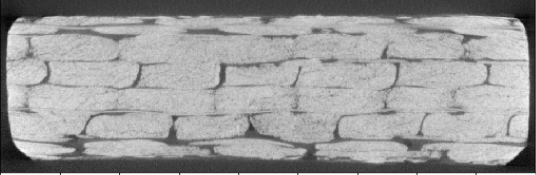
\includegraphics[width=\linewidth]{figures/Thibault/fibres_original.png}
		\caption{Original image.}
	\end{subfigure}
~
	\begin{subfigure}[b]{0.4\linewidth}
		\centering
		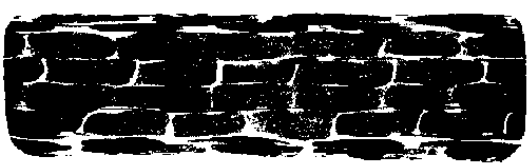
\includegraphics[width=\linewidth]{figures/Thibault/fibres_binar.png}
	\caption{Binarized image.}
\end{subfigure}
\label{fig:binar}
\end{figure}

\section{Morphological closing}

In order to have a clean image as much as possible, we tried to suppress the white dots the we can see in the binarized image.
Morphological operations can help to achieve this. They are based in using the context an image's pixel to change its value and perform some smoothing in the image.
Two operations are at the bases of morphological operations:
\begin{itemize}

\item{Dilation}\\\\
In dilation, a kernel of a specified size will slide on an image an put to 0 all pixels that have a 0 pixel under the kernel when the kernel is centered on it. Dilation operation correspond to dilating the white parts of an image like so:

\begin{minipage}{\linewidth}
	\centering
	
\includegraphics[width=5cm]{figures/Thibault/Morphology_1_Tutorial_Theory_Dilatation_2.png}
	\captionof{figure}{Exemple of dilation by a 3x3 kernel}
\end{minipage}

\item{Erosion}\\\\
Erosion would be the reverse operation where all pixels for which the kernel sees a black pixel when it is centerd on it is put to black:

\begin{minipage}{\linewidth}
	\centering
	
\includegraphics[width=5cm]{figures/Thibault/Morphology_1_Tutorial_Theory_Erosion_2.png}
	\captionof{figure}{Exemple of erosion by a 3x3 kernel}
\end{minipage}

\end{itemize}


We used a combination of dilation and erosion, known as morphological opening. The interest of this operation is that white dots
contained in the fibers will be merged to the fiber during the dilation and won't be changes back to white during erosion because
their context pixels will be black.

\begin{figure}[!h]
\centering
	\begin{subfigure}[b]{0.4\linewidth}
		\centering
		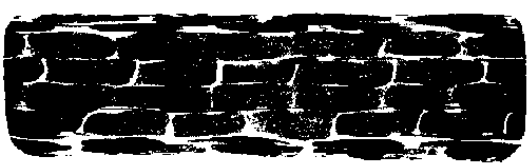
\includegraphics[width=\linewidth]{figures/Thibault/fibres_binar.png}
		\caption{Binarized image.}
	\end{subfigure}
~
	\begin{subfigure}[b]{0.4\linewidth}
		\centering
		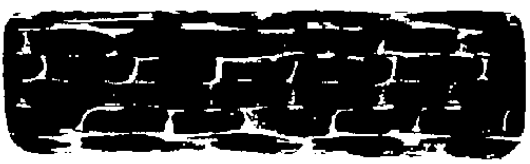
\includegraphics[width=\linewidth]{figures/Thibault/fibres_closed.png}
	\caption{Closed binarized image.}
\end{subfigure}
\label{fig:binar}
\end{figure}

\section{Annotations}

In order to have a few ground truth segmentations, we manually annotated a few, using this soft found on github\href{https://github.com/wkentaro/labelme}{here}.

VISU

We labeled 15 images equally distanced in the volume of 700 images.

\chapter{Classical segmentation methods}

There already exist several methods in image processing to segment images, mainly using the difference between different part of it to separate them.   
However, as we will see, they do not work very well on their own, mainly because of the fact that the edges are not clearly delimited.

\section{Filters}
\section{Watershed}
The watershed transformation treats the image it operates upon like a topographic map, with the brightness of each point representing its height, and finds the lines that run along the tops of ridges. The basins delimited by these ridges will then be considered as
seperate entities.\newline
To apply this method, it is required to have regions that will be the starting points of the basins.
\medskip
Classicaly, this is done by using the distance transformed map of the input image, which is defined as the 2d array
of the same size as the input image containing the distances of each pixel to its nearest white pixel.
\medskip\newline
Because of the rectangular shape of the fibers, we used the following distance on during this transformation:
$d((x_1,y_1),(x_2,y_2))=|x_1-x_2|+\alpha{|y_1-y_2|}$ where $\alpha$ is a parameter of the model.\newline
This makes the pixel where two fibers are horizontally overlapping have lower value than they would have had with an euclidian distance.

We then used the yen threshold to select the values that are high enough and indicate a potential basin of attraction for the watershed algorithm.
\begin{figure}[!h]
\centering
	\begin{subfigure}[b]{0.4\linewidth}
		\centering
		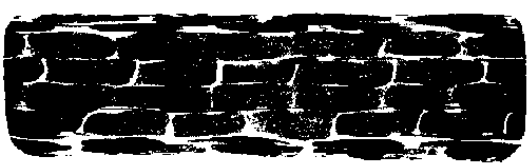
\includegraphics[width=\linewidth]{figures/Thibault/fibres_binar.png}
		\caption{Binarized image.}
	\end{subfigure}
~
	\begin{subfigure}[b]{0.4\linewidth}
		\centering
		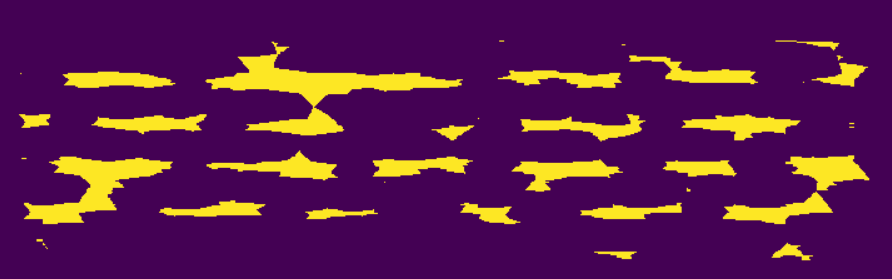
\includegraphics[width=\linewidth]{figures/Thibault/fibres_distance.png}
	\caption{Thresholded distance transformed image.}
\end{subfigure}
\label{fig:binar}
\end{figure}


We then used an implementation of the watershed algorithm to obtain the segmentation from \ref{fig:seg}

\begin{figure}[!h]
	\centering
	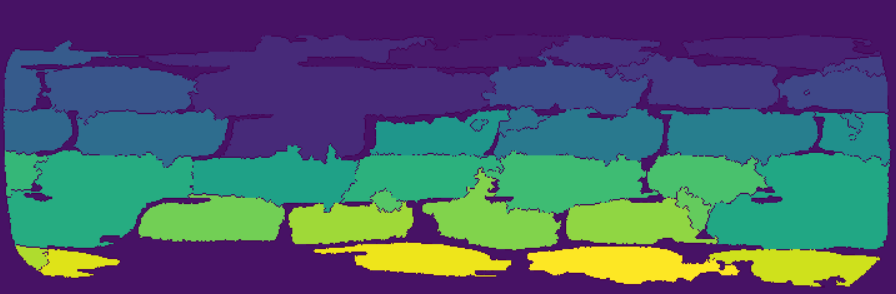
\includegraphics[width=9cm]{figures/Thibault/fibres_water.png}
	\caption{Watershed segmentation}
	\label{fig:seg}
\end{figure}

The algorithm shows good results. However it is still unable to separate fibers that overlap too much.\newline
We found a great sensitivity of the algorithm to the different threshold used.\newline
The threshold used to binarize the input image makes the algorithm detect lots of small portions if it is too high (because the fibers in the binarized image were burst in pieces), and large connected components if it is too low. On the other hand, the threshold on the distance transformed image acts in the opposite direction with high values causing few attraction basins detected by the algorithm and high values rendering lots of small pieces.
\section{Maximally Stable Extremal Regions}

The idea is to exploit the evolution of regions using different tresholds on an image. \newline

In fact, an increasing (or decreasing) tresholds on an image reveals growing areas of pixels that are below (or above) this treshold. The method consist in computing the area evolution rate of these regions and to consider that they are stable if this rate decreases. Therefore, this methods gives several "`stable"' regions on an image, and we can hope that they correspond to our bundles.  
However, this method need some tuning, notably the treshold changing rate, and we can use more informations like a bias on the area of the stable regions and their number.

Visu  
Equations

\chapter{Deep learning methods}

Our particular subject does not possess extensive litterature, but it has similarities with another one, the automatic cell detection on microscope images, which is more treated, and on which we concentrated our research.

The two mains categories of methods used in the litterature are roughly supervised and unsupervised methods.  \newline

In our case, supervised methods has a huge drawback. They need a lot of already annotated data to train them, which is not really doable here.  \newline

For unsupervised methods, we are trying to get informations from the data without any training set, which is our case.
In the case of deep learning an architecture enabling unsupervised training is an autoencoder. We mainly looked at 2 autoencoders and implemented them for our tests.\newline\newline
Another approach which could be promising would be to try to find a way to retrieve the missing edges, using for example the concavity of some curves in the image (cf...).\quadà mettre dans la partie d'au dessus ?

\section{W-net}

\section{Sparse autoencoder}
\subsection{architecture}
The authors of \cite{ref} used an encoder architecture to perform several tasks on cytoplasm images which contained several nuclei.
The different tasks they wanted to perform on these images were nuclei detection, nucei classification by cell type and nuclei segmentation.\newline

Their idea was to train a sparse autoencoder with a hidden layer that would contain the position of each nuclei as well a feature vector for each of them.
Therefore, the goal of the architecture is to have a 3-dimensional middle layer with most of its depthwise vectors being zeros as an encoding from which to reconstruct the image.
\begin{figure}[!h]
\centering
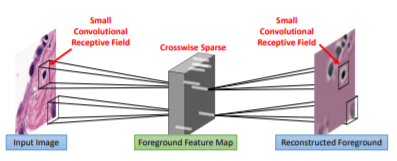
\includegraphics[width=7cm]{figures/Thibault/senc_hidden.png}
\caption{Encoder's hidden layer}
\end{figure}
\newline
The original architecture consists of a background encoding branch (lower branch of \ref{fig:arc}), a nuclei detection branch (middle branch of \ref{fig:arc}) and a local embedding branch that are convolutions that are point-wise multiplied with the detection map (upper branch of \ref{fig:arc})
\begin{figure}[!h]
\centering
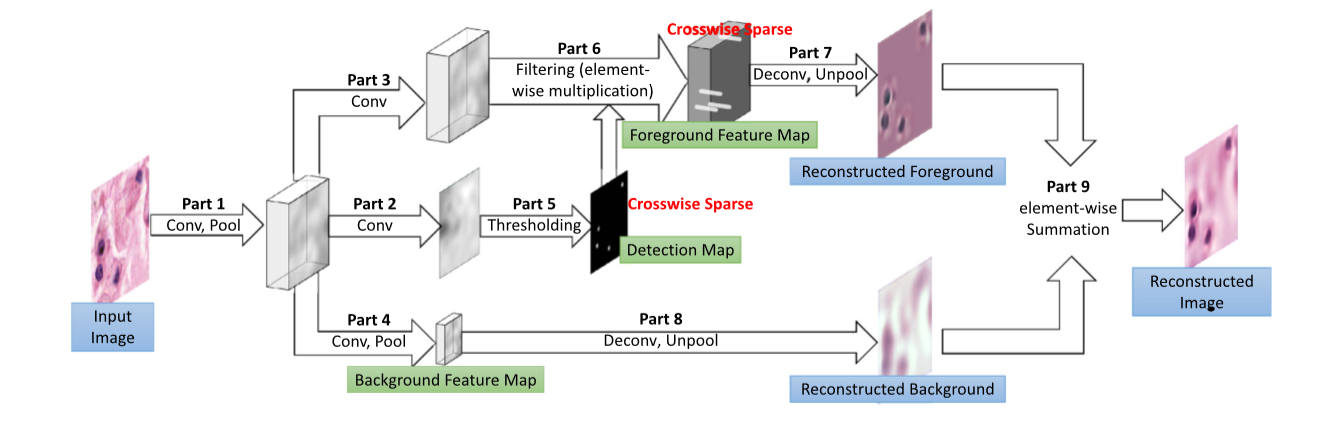
\includegraphics[width=17cm]{figures/Thibault/arc.png}
\caption{Encoder's architecture}
\label{fig:arc}
\end{figure}

\medskip
We tried to adapt this architecture to our problem.
Since the background of the images is almost constant in color, we got rid of the background encoding branch.
We also used less feature maps in the convolutions because the bricks we were trying to encode had less complexity than the original images.
In the section below, we detail a few implementation choices that we have made with this architecture.

\subsection{Implementation choices}
\begin{itemize}
\item{sparsity enforcement}
\medskip
\newline
The middle detection map is a 2D image that we want to be sparse with a predefined sparsity rate $\rho$\quad(we calculated the average density of
the fibers and derived the sparsity rate from it).\newline
To obtain this sparsity rate, we thresholded the detection map $D$ in a differentiable manner: $D'=\sigma(r(D-t_{\rho}))$

The way we found to calculate an appropriate threshold at batch level was to use a stochastic approximation.\newline
For a given 2D image from one sample, let $(X_n)$ be a flatten vector containg the values of its pixels, we take the last value of $\theta_n$ defined by $\theta_{n+1}=\theta_n-\frac{2}{n+1}*(1_{(X_{n+1}\le\theta_n)}-\rho)$\newline
We then average the values obtain on each sample of the batch.\newline
We also keep a running average of the thresholding value in memory for test time.
Thresholding with this value gave consistent sparsity rates when testing on random tensors.
\medskip
\item{Normalization}
\medskip
\newline
We found that keeping the values flowing in the network within a certain range was crucial.
To this end, we normalized the input tensor. We also used batch normalization between every layer which we found to be very usefull.
before the thresholding of the middle layer, we used batch normalization without mean and scale learnable parameters.
Indeed, we wanted the middle layer to have zero mean and unit variance to avoid it from lowering its variance via learnable scale parameter to have values within an ambiguous range of value of the sigmoid function (which we want to use as a thresholding function).
\end{itemize}
\subsection{Hyperparameters'influence}
We will detail some observation we made hyperparameters.
\newline
\bigskip
\begin{itemize}
\item{r (intensity of thresholding $D'=\sigma(r(D-t_{\rho}))$)}
\medskip
\newline
For the result we seek, we would think want this value to be as large as possible while avoiding exploding values during training.
However, we observed that the network was very keen on detecting some spots between the fibers and reconstruct the image from these.
This is what quickly happens when the thresholding was too hard.\newline
This may be due to a too powerfull architecture that allows the network to have the necessary informations to reconstruct the image from some points in between the cells, while the goal is to force it to use the informations about the simplest objects in the image
which are the brick shaped fibers.
\


\chapter{Methods tried}
We present here the methods that we actually implemented.

\section{Maximally stable Extremal Region}

We implemented the MSER algorithm as follows, adding a criteria on the minimal area of a component:
\begin{algorithm}
\caption{MSER implementation}
\begin{algorithmic} 
\STATE Starting treshold $tresh_{min}$
\STATE Maximum treshold $tresh_{max}$
\STATE Treshold step $tresh_{step}$
\STATE Minimal area $area_{min}$ 
\STATE Set of stopped components $Stopped_{Set}$ \newline

\STATE Current treshold $tresh_{current} = tresh_{min}$
\STATE We treshold the image and recover the connected components in $label_{current}$
\WHILE{$tresh_{current} \leq tresh_{max}$}
	\STATE $tresh_{current} \leftarrow tresh_{current} + tresh_{step}$
	\STATE We treshold the image and recover the new components in $label_{new}$
	\STATE We link the new labels with the old ones
	\STATE We compute the new growing rate
	\STATE Forall the new compoenntns, if the rate has decreased, we add them to stopped if the min area is reached otherwise we delete it
\ENDWHILE

\STATE Denominator $D \leftarrow 0$
\FOR{Each ground truth bundle $G_i$}
\STATE $j \leftarrow argmax_k J(G_i, S_k)$
\STATE $N \leftarrow N+|G_i\bigcap S_j|$
\STATE $D \leftarrow D+|G_i\bigcup S_j|$
\STATE Mark $S_j$ as used
\ENDFOR
\FOR{Each segmented bundle $S_k$}
\IF{$S_k$ has not been used}
\STATE $D \leftarrow D + |S_k|$
\ENDIF
\ENDFOR
\STATE $AJI \leftarrow N/D$
\end{algorithmic}
\end{algorithm}
  



\section{Sparse autoencoder}

\chapter{Results and discussion}
We present here our results.

\section{A few methods}
\section{Methods tried}
\subsection{etc}

\chapter{Conclusion}

\chapter{Bibliography}
REMPLIR

\bibliographystyle{plain}
\bibliography{biblio}
\end{document}
